\section{Bases ortonormales en $\r^n$}

\subsection{}

{\nologo
\begin{frame}\frametitle{Conjuntos ortogonales en $\r^n$}

\vspace{-2mm}
\begin{alertblock}{\textbf{Observación 1}}
	En $\r^3$ el conjunto de vectores de
	\[
	B = \Big\{ \, \underbrace{(1,0,0)}_{\color{blue}\mathbf{e}_1}, \ \underbrace{(0,1,0)}_{\color{blue}\mathbf{e}_2}, \ 
	\underbrace{(0,0,1)}_{\color{blue}\mathbf{e}_3} \, \Big\},
	\]
	satisface las siguientes propiedades:
	\begin{enumerate}
		\item[\labelname{$a$}] $\mathbf{e}_1\cdot \mathbf{e}_2 = 0$, $\mathbf{e}_1\cdot \mathbf{e}_3 = 0$ y $\mathbf{e}_2\cdot \mathbf{e}_3 = 0$.
		\item[\labelname{$b$}] $\Vert \mathbf{e}_1\Vert  = \Vert \mathbf{e}_2\Vert  = \Vert \mathbf{e}_3\Vert  = 1$.
	\end{enumerate}
\end{alertblock}

\vspace{-1mm}

\begin{defi}{\textbf{Definición 1}}\justifying
	Considere en $\r^n$ un conjunto de vectores
	\[
		S = \{ \mathbf{u}_1, \mathbf{u}_2, \hdots, \mathbf{u}_k\}.
	\]
	Se dice que:
	\begin{enumerate}
		\item[\labelname{$a$}] $S$ es  \textbf{\textit{ortogonal}} si cada par de vectores en $S$ distintos es ortogonal. %($\mathbf{u}_i\cdot \mathbf{u}_j=0, i\neq j$)
		\item[\labelname{$b$}] $S$ es \textbf{\textit{ortonormal}} si $S$ es ortogonal y cada vector en $S$ es \textbf{\textit{unitario}}.
	\end{enumerate}
	
\end{defi}	

%\begin{ej}{\textbf{Ejemplo 4}}
%	Encuentre el producto escalar de los vectores 
%	\[
%	\mathbf{u}=(1,2,0,-3) \qquad \text{y} \qquad \mathbf{v}=(3,-2,4,2).
%	\]
%\end{ej}

\end{frame}
}

%%------------------------------------------------------------------------------------------------------

\subsection{}

\begin{frame}\frametitle{Conjuntos ortogonales en $\r^n$}

%\begin{defi}{\textbf{Definición 1}}\justifying
%	Considere en $\r^n$ un conjunto de vectores
%	\[
%	S = \{ \mathbf{u}_1, \mathbf{u}_2, \hdots, \mathbf{u}_k\}.
%	\]
%	Se dice que:
%	\begin{enumerate}
%		\item[\labelname{$a$}] $S$ es  \textbf{\textit{ortogonal}} si cada par de vectores en $S$ distintos es ortogonal. %($\mathbf{u}_i\cdot \mathbf{u}_j=0, i\neq j$)
%		\item[\labelname{$b$}] $S$ es \textbf{\textit{ortonormal}} si $S$ es ortogonal y cada vector en $S$ es \textbf{\textit{unitario}}.
%	\end{enumerate}	
%\end{defi}	

\begin{ej}{\textbf{Ejemplo 1}}
	Muestre que el siguiente conjunto de vectores de $\r^3$ es ortonormal.
	\[
		S = \Bigg\{ \, \underbrace{\left( \frac{1}{\sqrt{2}}, \frac{1}{\sqrt{2}}, 0 \right)}_{\color{blue}\mathbf{v}_1}, \ 
		\underbrace{\left( -\frac{\sqrt{2}}{6}, \frac{\sqrt{2}}{6}, \frac{2\sqrt{2}}{3} \right)}_{\color{blue}\mathbf{v}_2}, \ 
		\underbrace{\left( \frac{2}{3}, -\frac{2}{3}, \frac{1}{3} \right)}_{\color{blue}\mathbf{v}_3} \, \Bigg\}.
	\]
\end{ej}
\textit{Solución}.

\end{frame}

%%------------------------------------------------------------------------------------------------------

\subsection{}

\begin{frame}\frametitle{Relación entre conjuntos ortogonales y LI}

\begin{defi}{\textbf{Definición 1}}\justifying
	Considere en $\r^n$ un conjunto de vectores
	\[
	S = \{ \mathbf{u}_1, \mathbf{u}_2, \hdots, \mathbf{u}_k\}.
	\]
	Se dice que:
	\begin{enumerate}
		\item[\labelname{$a$}] $S$ es  \textbf{\textit{ortogonal}} si cada par de vectores en $S$ distintos es ortogonal. %($\mathbf{u}_i\cdot \mathbf{u}_j=0, i\neq j$)
		\item[\labelname{$b$}] $S$ es \textbf{\textit{ortonormal}} si $S$ es ortogonal y cada vector en $S$ es \textbf{\textit{unitario}}.
	\end{enumerate}
	
\end{defi}	

\begin{prop}{\textbf{Propiedad 1}}
	\justifying
	Si $S = \{ \mathbf{u}_1, \mathbf{u}_2, \hdots, \mathbf{u}_k\}$ es un \textit{conjunto ortogonal} de vectores no nulos en $\r^n$, entonces
	$S$ es linealmente independiente.
\end{prop}	

%\begin{prop}{\textbf{Propiedad 2}}
%	\justifying
%	En $\r^n$ todo conjunto ortogonal de $n$ vectores es base.
%\end{prop}	

\end{frame}

%%------------------------------------------------------------------------------------------------------

\subsection{}

\begin{frame}\frametitle{Relación entre conjuntos ortogonales y LI}
	
	\begin{defi}{\textbf{Definición 1}}\justifying
		Considere en $\r^n$ un conjunto de vectores
		\[
		S = \{ \mathbf{u}_1, \mathbf{u}_2, \hdots, \mathbf{u}_k\}.
		\]
		Se dice que:
		\begin{enumerate}
			\item[\labelname{$a$}] $S$ es  \textbf{\textit{ortogonal}} si cada par de vectores en $S$ distintos es ortogonal. %($\mathbf{u}_i\cdot \mathbf{u}_j=0, i\neq j$)
			\item[\labelname{$b$}] $S$ es \textbf{\textit{ortonormal}} si $S$ es ortogonal y cada vector en $S$ es \textbf{\textit{unitario}}.
		\end{enumerate}
		
	\end{defi}	
	
%	\begin{prop}{\textbf{Propiedad 1}}
%		\justifying
%		Si $S = \{ \mathbf{u}_1, \mathbf{u}_2, \hdots, \mathbf{u}_k\}$ es un \textit{conjunto ortogonal} de vectores no nulos en $\r^n$, entonces
%		$S$ es linealmente independiente.
%	\end{prop}	
	
	\begin{prop}{\textbf{Propiedad 2}}
		\justifying
		En $\r^n$ todo conjunto ortogonal de $n$ vectores es base.
	\end{prop}	
	
\end{frame}

%%------------------------------------------------------------------------------------------------------

\subsection{}

\begin{frame}\frametitle{Relación entre conjuntos ortogonales y LI}

%\begin{prop}{\textbf{Propiedad 1}}
%	\justifying
%	Si $S = \{ \mathbf{u}_1, \mathbf{u}_2, \hdots, \mathbf{u}_k\}$ es un \textit{conjunto ortogonal} de vectores no nulos en $\r^n$, entonces
%	$S$ es linealmente independiente.
%\end{prop}	

\begin{prop}{\textbf{Propiedad 2}}
	\justifying
	En $\r^n$ todo conjunto ortogonal de $n$ vectores es base.
\end{prop}	

\begin{ej}{\textbf{Ejemplo 2}}
	Muestre que el siguiente conjunto de vectores es base para $\r^4$.
	\[
		S = \Big\{ \, \underbrace{(2,3,2,-2)}_{\color{blue}\mathbf{v}_1}, \ \underbrace{(1,0,0,1)}_{\color{blue}\mathbf{v}_2}, \ 
	\underbrace{(-1,0,2,1)}_{\color{blue}\mathbf{v}_3}, \ \underbrace{(-1,2,-1,1)}_{\color{blue}\mathbf{v}_4} \, \Big\},
	\]
\end{ej}
\textit{Solución}.

\end{frame}

%%------------------------------------------------------------------------------------------------------

\subsection{}

\begin{frame}\frametitle{Coeficientes de Fourier}
	
	\begin{prop}{\textbf{Propiedad 3}}
		\justifying
		Si $B = \{ \mathbf{v}_1, \mathbf{v}_2, \hdots, \mathbf{v}_n\}$ es un \textit{base ortogonal} para $\r^n$, entonces
		cada vector $\mathbf{w}$ en $\r^n$ se pude representar como
		\[
		\mathbf{w} = \left( \frac{\mathbf{w}\cdot \mathbf{v}_1}{\Vert \mathbf{v}_1 \Vert^2} \right)\, \mathbf{v}_1 + 
		\left( \frac{\mathbf{w}\cdot \mathbf{v}_2}{\Vert \mathbf{v}_2 \Vert^2} \right)\, \mathbf{v}_2 + \cdots 
		+ \left( \frac{\mathbf{w}\cdot \mathbf{v}_n}{\Vert \mathbf{v}_n \Vert^2} \right)\, \mathbf{v}_n.
		\]
		
		\vspace{-1mm}
	\end{prop}		

	\begin{alertblock}{\textbf{Observación 2}}		
		\[
			\mathbf{w} = \text{proy}_{\mathbf{v_1}} \mathbf{w} + \text{proy}_{\mathbf{v_2}} \mathbf{w} + \cdots +
			 			 \text{proy}_{\mathbf{v_n}} \mathbf{w}. 
		\]
	\end{alertblock}
	
\end{frame}

%%------------------------------------------------------------------------------------------------------

\subsection{}

\begin{frame}\frametitle{Coeficientes de Fourier}
	
	\begin{prop}{\textbf{Propiedad 4}}
		\justifying
		Si $B = \{ \mathbf{u}_1, \mathbf{u}_2, \hdots, \mathbf{u}_n\}$ es un \textit{base ortonormal} para $\r^n$, entonces
		cada vector $\mathbf{w}$ en $\r^n$ se pude representar como
		\[
		\mathbf{w} = (\mathbf{w}\cdot \mathbf{u}_1)\, \mathbf{u}_1 + (\mathbf{w}\cdot \mathbf{u}_2)\, \mathbf{u}_2 + \cdots 
		+ (\mathbf{w}\cdot \mathbf{u}_n)\, \mathbf{u}_n.
		\]
		
		\vspace{-1mm}
	\end{prop}		
	
\end{frame}

%%------------------------------------------------------------------------------------------------------

\subsection{}

{\nologo
\begin{frame}\frametitle{Coeficientes de Fourier}

\begin{prop}{\textbf{Propiedad 4}}
	\justifying
	Si $B = \{ \mathbf{u}_1, \mathbf{u}_2, \hdots, \mathbf{u}_n\}$ es un \textit{base ortonormal} para $\r^n$, entonces
	cada vector $\mathbf{w}$ en $\r^n$ se pude representar como
	\[
	\mathbf{w} = (\mathbf{w}\cdot \mathbf{u}_1)\, \mathbf{u}_1 + (\mathbf{w}\cdot \mathbf{u}_2)\, \mathbf{u}_2 + \cdots 
	+ (\mathbf{w}\cdot \mathbf{u}_n)\, \mathbf{u}_n.
	\]
	
	\vspace{-1mm}
\end{prop}		

\begin{alertblock}{\textbf{Observación 3}}	
	\begin{enumerate}\justifying
		\item[\labelname{$a$}] En la propiedad 3, a las coordenadas de $\mathbf{w}$ respecto a la base $B$ se les llama \textit{coeficientes de Fourier}
		de $\mathbf{w}$ respecto a $B$.
		\item[\labelname{$b$}] El vector de coordenadas de $\mathbf{w}$ respecto a al base $B$ es
		\[
		\left[ \mathbf{w} \right]_{\mathcal{B}} = 
		\left[
		\begin{array}{c}
		\mathbf{w}\cdot \mathbf{v}_1\\[1mm]
		\mathbf{w}\cdot \mathbf{v}_2\\[1mm]
		\vdots\\[2mm]
		\mathbf{w}\cdot \mathbf{v}_n
		\end{array}
		\right]
		\]
	\end{enumerate}
\end{alertblock}

\end{frame}
}

%%------------------------------------------------------------------------------------------------------

\subsection{}

\begin{frame}%\frametitle{Representación de vectores respecto a una base ortonormal}

\begin{prop}{\textbf{Propiedad 4}}
	\justifying
	Si $B = \{ \mathbf{u}_1, \mathbf{u}_2, \hdots, \mathbf{u}_n\}$ es un \textit{base ortonormal} para $\r^n$, entonces
	cada vector $\mathbf{w}$ en $\r^n$ se pude representar como
	\[
	\mathbf{w} = (\mathbf{w}\cdot \mathbf{u}_1)\, \mathbf{u}_1 + (\mathbf{w}\cdot \mathbf{u}_2)\, \mathbf{u}_2 + \cdots 
	+ (\mathbf{w}\cdot \mathbf{u}_n)\, \mathbf{u}_n.
	\]
	
	\vspace{-1mm}
\end{prop}		

\begin{ej}{\textbf{Ejemplo 3}}\justifying 
	Encuentre el vector de coordenadas de $\mathbf{w}=(5,-5,2)$ respecto a la base ortonormal
	\[
	B = \Bigg\{ \, \underbrace{\left( \frac{3}{5}, \frac{4}{5}, 0 \right)}_{\color{blue}\mathbf{v}_1}, \ 
	\underbrace{\left( -\frac{4}{5}, \frac{3}{5}, 0 \right)}_{\color{blue}\mathbf{v}_2}, \ 
	\underbrace{\Big( 0, 0, 1 \Big)}_{\color{blue}\mathbf{v}_3} \, \Bigg\}.
	\]
\end{ej}
\textit{Solución}.

\end{frame}

%%------------------------------------------------------------------------------------------------------

\subsection{}

{\nologo
\begin{frame}\frametitle{Proceso de ortonormalización de Gram-Schmidt en $\r^2$}

\vspace{-2mm}

\begin{center}
	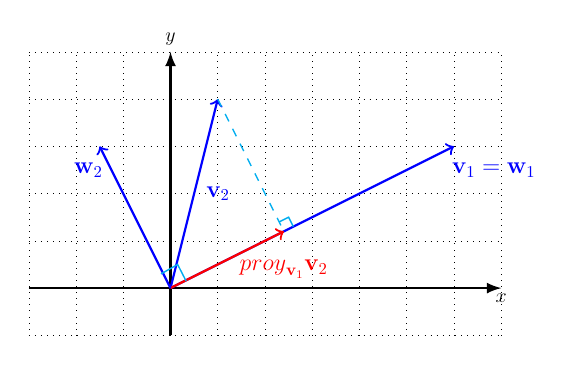
\begin{tikzpicture}[thick,scale=0.6, every node/.style={scale=0.6}]%[scale=.8,font=\scriptsize]
	\draw[help lines,black,dotted] (-3,-1) grid (7,5);
	\draw[thick,-latex] (-3,0) -- (7,0) node[below] {\large $x$};
	\draw[thick,-latex] (0,-1) -- (0,5) node[above] {\large $y$};	
	% vector v_1
	\draw [color=blue,->] (0,0) -- (6,3);
	%	\fill[color=blue,draw] (4,0.5) node[below,left] {\Large $\mathbf{u}$};
	\fill[color=blue,draw] (5.5,2.5) node[right] {\Large \ \  $\mathbf{v}_1 = \mathbf{w}_1$};
	% vector v_2
	\draw [color=blue,->] (0,0) -- (1,4);	
	\fill[color=blue,draw] (0.3,2) node[right] {\Large \ \  $\mathbf{v}_2$};
	\draw [color=cyan,line width=0.18mm,dashed,-] (1,4) -- (2.4,1.2);
	\draw [color=cyan,line width=0.18mm,-] (2.3,1.4) -- (2.5,1.5) -- (2.6,1.3);
	% vector proy_v_1 v_2
	\draw [color=red,->] (0,0) -- (2.4,1.2);
	\fill[color=red,draw] (1,0.4) node[right] {\Large \ \  $\text{proy}_{\mathbf{v}_1} \mathbf{v}_2$};
	% vector proy_w_2
	\draw [color=blue,->] (0,0) -- (-1.5,3);
	\fill[color=blue,draw] (-2.5,2.5) node[right] {\Large \ \  $ \mathbf{w}_2$};
	\draw [color=cyan,line width=0.18mm,-] (-0.2,0.3) -- (0.15,0.5) -- (0.33,0.15);
	%	\draw [line width=0.1mm,color=blue,dashed,-] (5,0) -- (5,2);
	%	\fill[color=blue,draw] (5,0) node[below] {\Large $v_1$};
	%	\draw [line width=0.1mm,color=blue,dashed,-] (0,2) -- (5,2);	
	%	\fill[color=blue,draw] (0,2) node[left] {\Large $v_2$};
	% vector v
%	\draw [color=blue,->] (4,1) -- (5,5);
	%	\fill[color=blue,draw] (4.8,4.8) node[right] {\Large \ \  $\mathbf{v}$};
%	\fill[color=blue,draw] (4.3,2.8) node[rotate=0,right] {\Large \ \  $\Vert\mathbf{v}\Vert$};
	%	\draw [line width=0.15mm,color=red,dashed,-] (5,2) -- (-4,5);	
	%	\fill[color=red,draw] (1.8,3.5) node[rotate=-20,left] {\Large $d(\mathbf{u}, \mathbf{v})$};	
	\end{tikzpicture}
\end{center}

\begin{prop}{\textbf{Propiedad 4 (Gram-Schmidt)}}
	\justifying
	Si $\{\mathbf{v}_1, \mathbf{v}_2\}$ es una base de $\r^2$, entonces los vectores $\mathbf{w}_1$ y $\mathbf{w}_2$ dados por
	\[
	\begin{array}{rcl}
		\mathbf{w}_1 & = & \mathbf{v}_1 \\
		\mathbf{w}_2 & = & \mathbf{v}_2 - \text{proy}_{\mathbf{w}_1} \mathbf{v}_2 \ = \ \mathbf{v}_2 - 
		                    \dfrac{\mathbf{v}_2\cdot \mathbf{w}_1}{\Vert \mathbf{w}_1 \Vert^2}\ \mathbf{w}_1\\
	\end{array}
	\]
	forman una base \textit{ortogonal} de $\r^2$.
\end{prop}	

\end{frame}
}

%%------------------------------------------------------------------------------------------------------

\subsection{}

\begin{frame}%\frametitle{Proceso de ortonormalización de Gram-Schmidt en $\r^2$}

\begin{prop}{\textbf{Propiedad 4 (Gram-Schmidt)}}
	\justifying
	Si $\{\mathbf{v}_1, \mathbf{v}_2\}$ es una base de $\r^2$, entonces los vectores $\mathbf{w}_1$ y $\mathbf{w}_2$ dados por
	\[
	\begin{array}{rcl}
	\mathbf{w}_1 & = & \mathbf{v}_1 \\
	\mathbf{w}_2 & = & \mathbf{v}_2 - \text{proy}_{\mathbf{w}_1} \mathbf{v}_2 \ = \ \mathbf{v}_2 - 
	\dfrac{\mathbf{v}_2\cdot \mathbf{w}_1}{\Vert \mathbf{w}_1 \Vert^2}\ \mathbf{w}_1
	\end{array}
	\]
	forman una base \textit{ortogonal} de $\r^2$.
\end{prop}	

\begin{ej}{\textbf{Ejemplo 4}}\justifying 
	Aplique el proceso de ortonormalización de Gram-Schmidt a la siguiente base de $\r^2$:
	\[
	B = \Big\{ \, \underbrace{(1,1)}_{\color{blue}\mathbf{v}_1}, \ \underbrace{(0,1)}_{\color{blue}\mathbf{v}_2} \, \Big\},
	\]
\end{ej}
\textit{Solución}.

\end{frame}

%%------------------------------------------------------------------------------------------------------

\subsection{}

{\nologo
\begin{frame}\frametitle{Proceso de ortonormalización de Gram-Schmidt en $\r^n$}

\vspace{-4mm}

\begin{prop}{\textbf{Propiedad 5 (Gram-Schmidt en $\r^n$)}}
	\justifying
	\begin{enumerate}
		\item Sea $\{\mathbf{v}_1,\hdots, \mathbf{v}_n\}$ es una base de $\r^n$.
		
		\item Definimos ${\color{blue}\mathbf{w}_1},{\color{blue}\mathbf{w}_2},\hdots, {\color{blue}\mathbf{w}_n}$ como
		\[
		\begin{array}{r@{\hspace{0.5\tabcolsep}}c@{\hspace{0.5\tabcolsep}}l}
		{\color{blue}\mathbf{w}_1} & = & {\color{blue}\mathbf{v}_1} \\[2mm]
		{\color{blue}\mathbf{w}_2} & = & \mathbf{v}_2 - \text{proy}_{\mathbf{w}_1} \mathbf{v}_2 \ = \ {\color{blue} \mathbf{v}_2 - 
		\dfrac{\mathbf{v}_2\cdot \mathbf{w}_1}{\Vert \mathbf{w}_1 \Vert^2}\ \mathbf{w}_1 } \\[5mm]
		{\color{blue}\mathbf{w}_3} & = & \mathbf{v}_3 - \text{proy}_{\mathbf{w}_1} \mathbf{v}_3 - \text{proy}_{\mathbf{w}_2} \mathbf{v}_3 \ = \ 
		{\color{blue} \mathbf{v}_3 - \dfrac{\mathbf{v}_3\cdot \mathbf{w}_1}{\Vert \mathbf{w}_1 \Vert^2}\ \mathbf{w}_1
		- \dfrac{\mathbf{v}_3\cdot \mathbf{w}_2}{\Vert \mathbf{w}_2 \Vert^2}\ \mathbf{w}_2 } \\[0mm]
		& \vdots & \\
		{\color{blue}\mathbf{w}_n} & = & {\color{blue} \mathbf{v}_n - \dfrac{\mathbf{v}_n\cdot \mathbf{w}_1}{\Vert \mathbf{w}_1 \Vert^2}\ \mathbf{w}_1 - \dfrac{\mathbf{v}_n\cdot \mathbf{w}_2}{\Vert \mathbf{w}_2 \Vert^2}\ \mathbf{w}_2 - \cdots
								- \dfrac{\mathbf{v}_n\cdot \mathbf{w}_{n-1}}{\Vert \mathbf{w}_{n-1} \Vert^2}\ \mathbf{w}_{n-1} }
		\end{array}
		\]
		Entonces el conjunto $\{{\color{blue}\mathbf{w}_1},{\color{blue}\mathbf{w}_2},\hdots, {\color{blue}\mathbf{w}_n}\}$ es una base \textit{ortogonal} para $\r^n$.
		
%		\vspace{2mm}
		\item Definimos ${\color{red}\mathbf{u}_i} = \frac{{\color{blue}\mathbf{w}_i}}{\Vert {\color{blue}\mathbf{w}_i} \Vert}$ y entonces el conjunto
		\[
			\{{\color{red}\mathbf{u}_1},{\color{red}\mathbf{u}_2},\hdots, {\color{red}\mathbf{u}_n}\}
		\]
		es una base \textit{ortonormal} de $\r^n$.
	\end{enumerate}
\end{prop}	

\end{frame}
}

%%------------------------------------------------------------------------------------------------------

\subsection{}

{\nologo
\begin{frame}\frametitle{Proceso de ortonormalización de Gram-Schmidt en $\r^n$}

\begin{prop}{}%{\textbf{Propiedad 8 (Gram-Schmidt en $\r^n$)}}
	
	\vspace{-4mm}
	\[
	\begin{array}{r@{\hspace{0.5\tabcolsep}}c@{\hspace{0.5\tabcolsep}}l}
	{\color{blue}\mathbf{w}_1} & = & {\color{blue}\mathbf{v}_1} \\[2mm]
	{\color{blue}\mathbf{w}_2} & = & \mathbf{v}_2 - \text{proy}_{\mathbf{w}_1} \mathbf{v}_2 \ = \ {\color{blue} \mathbf{v}_2 - 
		\dfrac{\mathbf{v}_2\cdot \mathbf{w}_1}{\Vert \mathbf{w}_1 \Vert^2}\ \mathbf{w}_1 } \\[5mm]
	{\color{blue}\mathbf{w}_3} & = & \mathbf{v}_3 - \text{proy}_{\mathbf{w}_1} \mathbf{v}_3 - \text{proy}_{\mathbf{w}_2} \mathbf{v}_3 \ = \ 
	{\color{blue} \mathbf{v}_3 - \dfrac{\mathbf{v}_3\cdot \mathbf{w}_1}{\Vert \mathbf{w}_1 \Vert^2}\ \mathbf{w}_1
		- \dfrac{\mathbf{v}_3\cdot \mathbf{w}_2}{\Vert \mathbf{w}_2 \Vert^2}\ \mathbf{w}_2 } \\[0mm]
	& \vdots & \\[2mm]
	{\color{blue}\mathbf{w}_n} & = & {\color{blue} \mathbf{v}_n - \dfrac{\mathbf{v}_n\cdot \mathbf{w}_1}{\Vert \mathbf{w}_1 \Vert^2}\ \mathbf{w}_1 - \dfrac{\mathbf{v}_n\cdot \mathbf{w}_2}{\Vert \mathbf{w}_2 \Vert^2}\ \mathbf{w}_2 - \cdots
		- \dfrac{\mathbf{v}_n\cdot \mathbf{w}_{n-1}}{\Vert \mathbf{w}_{n-1} \Vert^2}\ \mathbf{w}_{n-1} }
	\end{array}
	\]
\end{prop}	

\begin{ej}{\textbf{Ejemplo 5}}\justifying 
	Aplique el proceso de ortonormalización de Gram-Schmidt a la siguiente base de $\r^3$:
	\[
	B = \Big\{ \, \underbrace{(1,1,0)}_{\color{blue}\mathbf{v}_1}, \ \underbrace{(1,2,0)}_{\color{blue}\mathbf{v}_2}
	           , \ \underbrace{(0,1,2)}_{\color{blue}\mathbf{v}_3} \, \Big\}.
	\]
\end{ej}

\end{frame}
}

%%------------------------------------------------------------------------------------------------------

\subsection{}

\begin{frame}%\frametitle{Proyección ortogonal}

\begin{defi}{\textbf{Definición 2}}
	\justifying
	Suponga que $H$ es un subespacio de $\r^n$ con base \textit{ortogonal} 
	\[
		B = \{ \mathbf{v}_1, \mathbf{v}_2, \hdots, \mathbf{v}_k\}.
	\]
	Si $\mathbf{v}$ es un vector en $\r^n$, entonces la \textbf{\textit{proyección ortogonal}} de $\mathbf{v}$ sobre $H$
	es el vector definido por
	\[
		\text{proy}_H \mathbf{v} = \left( \frac{\mathbf{v}\cdot \mathbf{v}_1}{\Vert \mathbf{v}_1 \Vert^2} \right)\, \mathbf{v}_1 + 
		\left( \frac{\mathbf{v}\cdot \mathbf{v}_2}{\Vert \mathbf{v}_2 \Vert^2} \right)\, \mathbf{v}_2 + \cdots 
		+ \left( \frac{\mathbf{v}\cdot \mathbf{v}_k}{\Vert \mathbf{v}_k \Vert^2} \right)\, \mathbf{v}_k.
	\]
	
	\vspace{-1mm}
\end{defi}	

	\begin{alertblock}{\textbf{Observación 4}}
	\[
		\text{proy}_H \mathbf{v} = \text{proy}_{\mathbf{v_1}} \mathbf{v} + \text{proy}_{\mathbf{v_2}} \mathbf{v} + \cdots +
		\text{proy}_{\mathbf{v_k}} \mathbf{v}. 
	\]
\end{alertblock}

\end{frame}

%%------------------------------------------------------------------------------------------------------

\subsection{}

{\nologo
\begin{frame}%\frametitle{Proyección ortogonal}
	
	\begin{defi}{\textbf{Definición 2}}
		\justifying
		Suponga que $H$ es un subespacio de $\r^n$ con base \textit{ortogonal} 
		\[
		B = \{ \mathbf{v}_1, \mathbf{v}_2, \hdots, \mathbf{v}_k\}.
		\]
		Si $\mathbf{v}$ es un vector en $\r^n$, entonces la \textbf{\textit{proyección ortogonal}} de $\mathbf{v}$ sobre $H$
		es el vector definido por
		\[
		\text{proy}_H \mathbf{v} = \left( \frac{\mathbf{v}\cdot \mathbf{v}_1}{\Vert \mathbf{v}_1 \Vert^2} \right)\, \mathbf{v}_1 + 
		\left( \frac{\mathbf{v}\cdot \mathbf{v}_2}{\Vert \mathbf{v}_2 \Vert^2} \right)\, \mathbf{v}_2 + \cdots 
		+ \left( \frac{\mathbf{v}\cdot \mathbf{v}_k}{\Vert \mathbf{v}_k \Vert^2} \right)\, \mathbf{v}_k.
		\]
		
		\vspace{-1mm}
	\end{defi}	
	
	\begin{ej}{\textbf{Ejemplo 6}}\justifying 
		Encuentre la \textit{proyección ortogonal} del vector $\mathbf{v}=(1,1,3)$ de $\r^3$ sobre el subespacio generado por los vectores
		\[
		\mathbf{w}_1 = (0,3,1) \qquad \text{y} \qquad \mathbf{w}_2 = (2,0,0).
		\]
	\end{ej}
	\textit{Solución}.
	
\end{frame}
}

%%------------------------------------------------------------------------------------------------------

\subsection{}

{\nologo
\begin{frame}\frametitle{Proyección ortogonal}

\vspace{-3mm}	
\begin{defi}{\textbf{Definición 2}}
	\justifying
	Suponga que $H$ es un subespacio de $\r^n$ con base \textit{ortogonal} 
	\[
	B = \{ \mathbf{v}_1, \mathbf{v}_2, \hdots, \mathbf{v}_k\}.
	\]
	Si $\mathbf{v}$ es un vector en $\r^n$, entonces la \textbf{\textit{proyección ortogonal}} de $\mathbf{v}$ sobre $H$
	es el vector definido por
	\[
	\text{proy}_H \mathbf{v} = \left( \frac{\mathbf{v}\cdot \mathbf{v}_1}{\Vert \mathbf{v}_1 \Vert^2} \right)\, \mathbf{v}_1 + 
	\left( \frac{\mathbf{v}\cdot \mathbf{v}_2}{\Vert \mathbf{v}_2 \Vert^2} \right)\, \mathbf{v}_2 + \cdots 
	+ \left( \frac{\mathbf{v}\cdot \mathbf{v}_k}{\Vert \mathbf{v}_k \Vert^2} \right)\, \mathbf{v}_k.
	\]
	
	\vspace{-1mm}
\end{defi}	

\vspace{-1mm}

\begin{prop}{\textbf{Propiedad 6}}
	\justifying
	Suponga que $S$ es un subespacio de $\r^n$ y $\mathbf{v}$ un vector en $\r^n$. Entonces 
	
	\vspace{-5mm}	
	\begin{columns}
		\begin{column}{0.4\textwidth}
			\begin{figure}
				\centering
				\includegraphics[width=4cm]{imagenes/proyeccion}
			\end{figure}
		\end{column}
		\begin{column}{0.5\textwidth}  %%<--- here

			\vspace{2mm}
			\[
			\left\Vert \mathbf{v} - \text{proy}_S \mathbf{v} \right\Vert \leq 
			\left\Vert \mathbf{v} - \mathbf{u} \right\Vert
			\]		
			
			\vspace{4mm}
			para todo vector $\mathbf{u}$ en $S$.
		\end{column}
	\end{columns}
\end{prop}	
	
\end{frame}
}

%%------------------------------------------------------------------------------------------------------

\subsection{}

{\nologo
\begin{frame}\frametitle{Proyección ortogonal}

\begin{defi}{\textbf{Definición 2}}
	\justifying
	Suponga que $H$ es un subespacio de $\r^n$ con base \textit{ortogonal} 
	\[
	B = \{ \mathbf{v}_1, \mathbf{v}_2, \hdots, \mathbf{v}_k\}.
	\]
	Si $\mathbf{v}$ es un vector en $\r^n$, entonces la \textbf{\textit{proyección ortogonal}} de $\mathbf{v}$ sobre $H$
	es el vector definido por
	\[
	\text{proy}_H \mathbf{v} = \left( \frac{\mathbf{v}\cdot \mathbf{v}_1}{\Vert \mathbf{v}_1 \Vert^2} \right)\, \mathbf{v}_1 + 
	\left( \frac{\mathbf{v}\cdot \mathbf{v}_2}{\Vert \mathbf{v}_2 \Vert^2} \right)\, \mathbf{v}_2 + \cdots 
	+ \left( \frac{\mathbf{v}\cdot \mathbf{v}_k}{\Vert \mathbf{v}_k \Vert^2} \right)\, \mathbf{v}_k.
	\]
	
	\vspace{-1mm}
\end{defi}	

\begin{prop}{\textbf{Propiedad 7}}
	\justifying
	Suponga que $B = \{ \mathbf{u}_1, \mathbf{u}_2, \hdots, \mathbf{u}_n\}$ es una \textit{base ortonormal} para $\r^n$ y que
	$\mathbf{v}$ es un vector en $\r^n$. Entonces 
	\[
	\mathbf{v} = (\mathbf{v}\cdot \mathbf{u}_1)\, \mathbf{u}_1 + (\mathbf{v}\cdot \mathbf{u}_2)\, \mathbf{u}_2 + \cdots 
	+ (\mathbf{u}\cdot \mathbf{u}_n)\, \mathbf{u}_n.
	\]
	Es decir, $\text{proy}_{\rn} \mathbf{v} = \mathbf{v}$.
\end{prop}	

\end{frame}
}

%%------------------------------------------------------------------------------------------------------

\subsection{}

\begin{frame}\frametitle{Proyección ortogonal}
	
	\begin{ej}{\textbf{Ejemplo 7}}\justifying 
		Considere los siguientes subespacios de $\r^3$:
		\[
		H_1 = \text{gen} \{ (-1,1,1)\} \qquad \text{y} \qquad H_2 = \text{gen} \{ (1,0,1),(1,1,0)\}.
		\]
		Demuestre que todos los vectores de $H_1$ son ortogonales a todos los vectores de $H_2$.
		En tal caso se dice que los subespacios $H_1$ y $H_2$ son ortogonales.
	\end{ej}
	\textit{Solución}.	
	
\end{frame}

%%------------------------------------------------------------------------------------------------------

\subsection{}

\begin{frame}%\frametitle{Complemento ortogonal}

\begin{defi}{\textbf{Definición 3}}
	\justifying
	Suponga que $H$ es un subespacio de $\r^n$. El \textbf{\textit{complemento ortogonal}} de $H$ es el conjunto denotado
	por $H^{\perp}$ y definido como
	\[
		H^{\perp} = \{ \mathbf{x}\in\r^n \mid  \mathbf{x}\cdot \mathbf{h}=0 \text{ para todo } \mathbf{h}\in H \}
	\]
	
	\vspace{-1mm}
\end{defi}	

\begin{ej}{\textbf{Ejemplo 8}}\justifying 
	Encuentre el complemento ortogonal del subespacio $H$ de $\r^4$ generado por las columnas de la matriz
	\[
	A = 
	\left(
	\begin{array}{cc}
		1 & 0 \\[1mm]
		2 & 0 \\[1mm]
		1 & 0 \\[1mm]
		0 & 1 \\[1mm]
	\end{array}
	\right)
	\]
\end{ej}
\textit{Solución}.

\end{frame}

%%------------------------------------------------------------------------------------------------------

\subsection{}

\begin{frame}\frametitle{Complemento ortogonal}
	
	\begin{defi}{\textbf{Definición 3}}
		\justifying
		Suponga que $H$ es un subespacio de $\r^n$. El \textbf{\textit{complemento ortogonal}} de $H$ es el conjunto denotado
		por $H^{\perp}$ y definido como
		\[
		H^{\perp} = \{ \mathbf{x}\in\r^n \mid  \mathbf{x}\cdot \mathbf{h}=0 \text{ para todo } \mathbf{h}\in H \}
		\]
		
		\vspace{-1mm}
	\end{defi}	
	
	\begin{prop}{\textbf{Propiedad 8}}
		\justifying Suponga que $H$ es un subespacio de $\r^n$. Entonces
		
		\vspace{-2mm}
		\begin{multicols}{2}
			\begin{enumerate}\justifying
				\item[\labelname{$a$}] $H^{\perp}$ es un subespacio de $\r^n$.
				\item[\labelname{$b$}] $H\cap H^{\perp} = \{ \mathbf{0}\}$.
				\item[\labelname{$c$}] $\dim H + \dim H^{\perp} = n$.
			\end{enumerate}
		\end{multicols}
		
		\vspace{-3mm}
	\end{prop}	


		
\end{frame}

%%------------------------------------------------------------------------------------------------------

\subsection{}

\begin{frame}\frametitle{Complemento ortogonal}
	
	\begin{defi}{\textbf{Definición 3}}
		\justifying
		Suponga que $H$ es un subespacio de $\r^n$. El \textbf{\textit{complemento ortogonal}} de $H$ es el conjunto denotado
		por $H^{\perp}$ y definido como
		\[
		H^{\perp} = \{ \mathbf{x}\in\r^n \mid  \mathbf{x}\cdot \mathbf{h}=0 \text{ para todo } \mathbf{h}\in H \}
		\]
		
		\vspace{-1mm}
	\end{defi}	
	
	\begin{prop}{\textbf{Propiedad 9}}
		Suponga que $A$ es una matriz $m\times n$. Entonces		
		\begin{enumerate}[$a$]\justifying
			\item ${C_A}^{\perp} = N_{A^T}$.
			\item ${N_{A}}^{\perp} = R_{A}$.
		\end{enumerate}
	\end{prop}	
	
\end{frame}

%%------------------------------------------------------------------------------------------------------

\subsection{}

\begin{frame}\frametitle{Complemento ortogonal}
	
	\begin{defi}{\textbf{Definición 3}}
		\justifying
		Suponga que $H$ es un subespacio de $\r^n$. El \textbf{\textit{complemento ortogonal}} de $H$ es el conjunto denotado
		por $H^{\perp}$ y definido como
		\[
		H^{\perp} = \{ \mathbf{x}\in\r^n \mid  \mathbf{x}\cdot \mathbf{h}=0 \text{ para todo } \mathbf{h}\in H \}
		\]
		
		\vspace{-1mm}
	\end{defi}	
	
%	\begin{prop}{\textbf{Propiedad 8}}
%		\justifying Suponga que $H$ es un subespacio de $\r^n$. Entonces
%		
%		\vspace{-2mm}
%		\begin{multicols}{2}
%			\begin{enumerate}\justifying
%				\item[\labelname{$a$}] $H^{\perp}$ es un subespacio de $\r^n$.
%				\item[\labelname{$b$}] $H\cap H^{\perp} = \{ \mathbf{0}\}$.
%				\item[\labelname{$c$}] $\dim H + \dim H^{\perp} = n$.
%			\end{enumerate}
%		\end{multicols}
%		
%		\vspace{-3mm}
%	\end{prop}	
	
	\begin{prop}{\textbf{Propiedad 10 (Teorema de la proyección)}}
		\justifying Suponga que $H$ es un subespacio de $\r^n$. Entonces para cada vector $\mathbf{v}$ en $\r^n$
		existen vectores únicos $\mathbf{p}$ en $H$ y $\mathbf{q}$ en $H^{\perp}$ tales que 
		\[
			\mathbf{v} = \mathbf{p} + \mathbf{q} = \text{proy}_H \mathbf{v} + \text{proy}_{H^{\perp}} \mathbf{v}
		\]
		
	\end{prop}	
	
\end{frame}

%%------------------------------------------------------------------------------------------------------

\subsection{}

\begin{frame}%\frametitle{Complemento ortogonal}
	
	\begin{ej}{\textbf{Ejemplo 9}}\justifying 
		Sea $H$ el subespacio de $\r^4$ que tiene como base a las columnas de  
		\[
		A = 
		\left(
		\begin{array}{rrr}
		1 & 1 & 3 \\[1mm]
		1 & -1 & 2 \\[1mm]
		1 & 0 & 1 \\[1mm]
		0 & 1 & 2 
		\end{array}
		\right)
		\]
		\begin{enumerate}
			\item[\labelname{$a$}] Halle una base ortogonal para $H$.
		\end{enumerate}
	\end{ej}
	\textit{Solución.}
	
\end{frame}

%%------------------------------------------------------------------------------------------------------

\subsection{}

\begin{frame}%\frametitle{Complemento ortogonal}
	
	\begin{ej}{\textbf{Ejemplo 9}}\justifying 
		Sea $H$ el subespacio de $\r^4$ que tiene como base a las columnas de  
		\[
		A = 
		\left(
		\begin{array}{rrr}
		1 & 1 & 3 \\[1mm]
		1 & -1 & 2 \\[1mm]
		1 & 0 & 1 \\[1mm]
		0 & 1 & 2 
		\end{array}
		\right)
		\]
		\begin{enumerate}
			\item[\labelname{$b$}] Halle $\text{proy}_H \mathbf{v}$, donde $\mathbf{v}=(-2,0,2,2)$.
		\end{enumerate}
	\end{ej}
	\textit{Solución.}
	
\end{frame}

%%------------------------------------------------------------------------------------------------------

\subsection{}

\begin{frame}%\frametitle{Complemento ortogonal}
	
	\begin{ej}{\textbf{Ejemplo 9}}\justifying 
		Sea $H$ el subespacio de $\r^4$ que tiene como base a las columnas de  
		\[
		A = 
		\left(
		\begin{array}{rrr}
		1 & 1 & 3 \\[1mm]
		1 & -1 & 2 \\[1mm]
		1 & 0 & 1 \\[1mm]
		0 & 1 & 2 
		\end{array}
		\right)
		\]
		\begin{enumerate}
			\item[\labelname{$c$}] Halle $H^{\perp}$.
		\end{enumerate}
	\end{ej}
	\textit{Solución.}
	
\end{frame}
